\documentclass{article}

\usepackage{graphicx}
\usepackage{tikz}
\usepackage{tikzsymbols}
\usetikzlibrary{calc,patterns,shapes.geometric}
\pagestyle{empty}
\usepackage[margin=0pt]{geometry}
\geometry{papersize={14in,12in}}

\def\centerarc[#1](#2)(#3:#4:#5){\draw[#1] ($(#2)+({#5*cos(#3)},{#5*sin(#3)})$) arc (#3:#4:#5);}

\begin{document}
	\begin{figure}
		\centering
		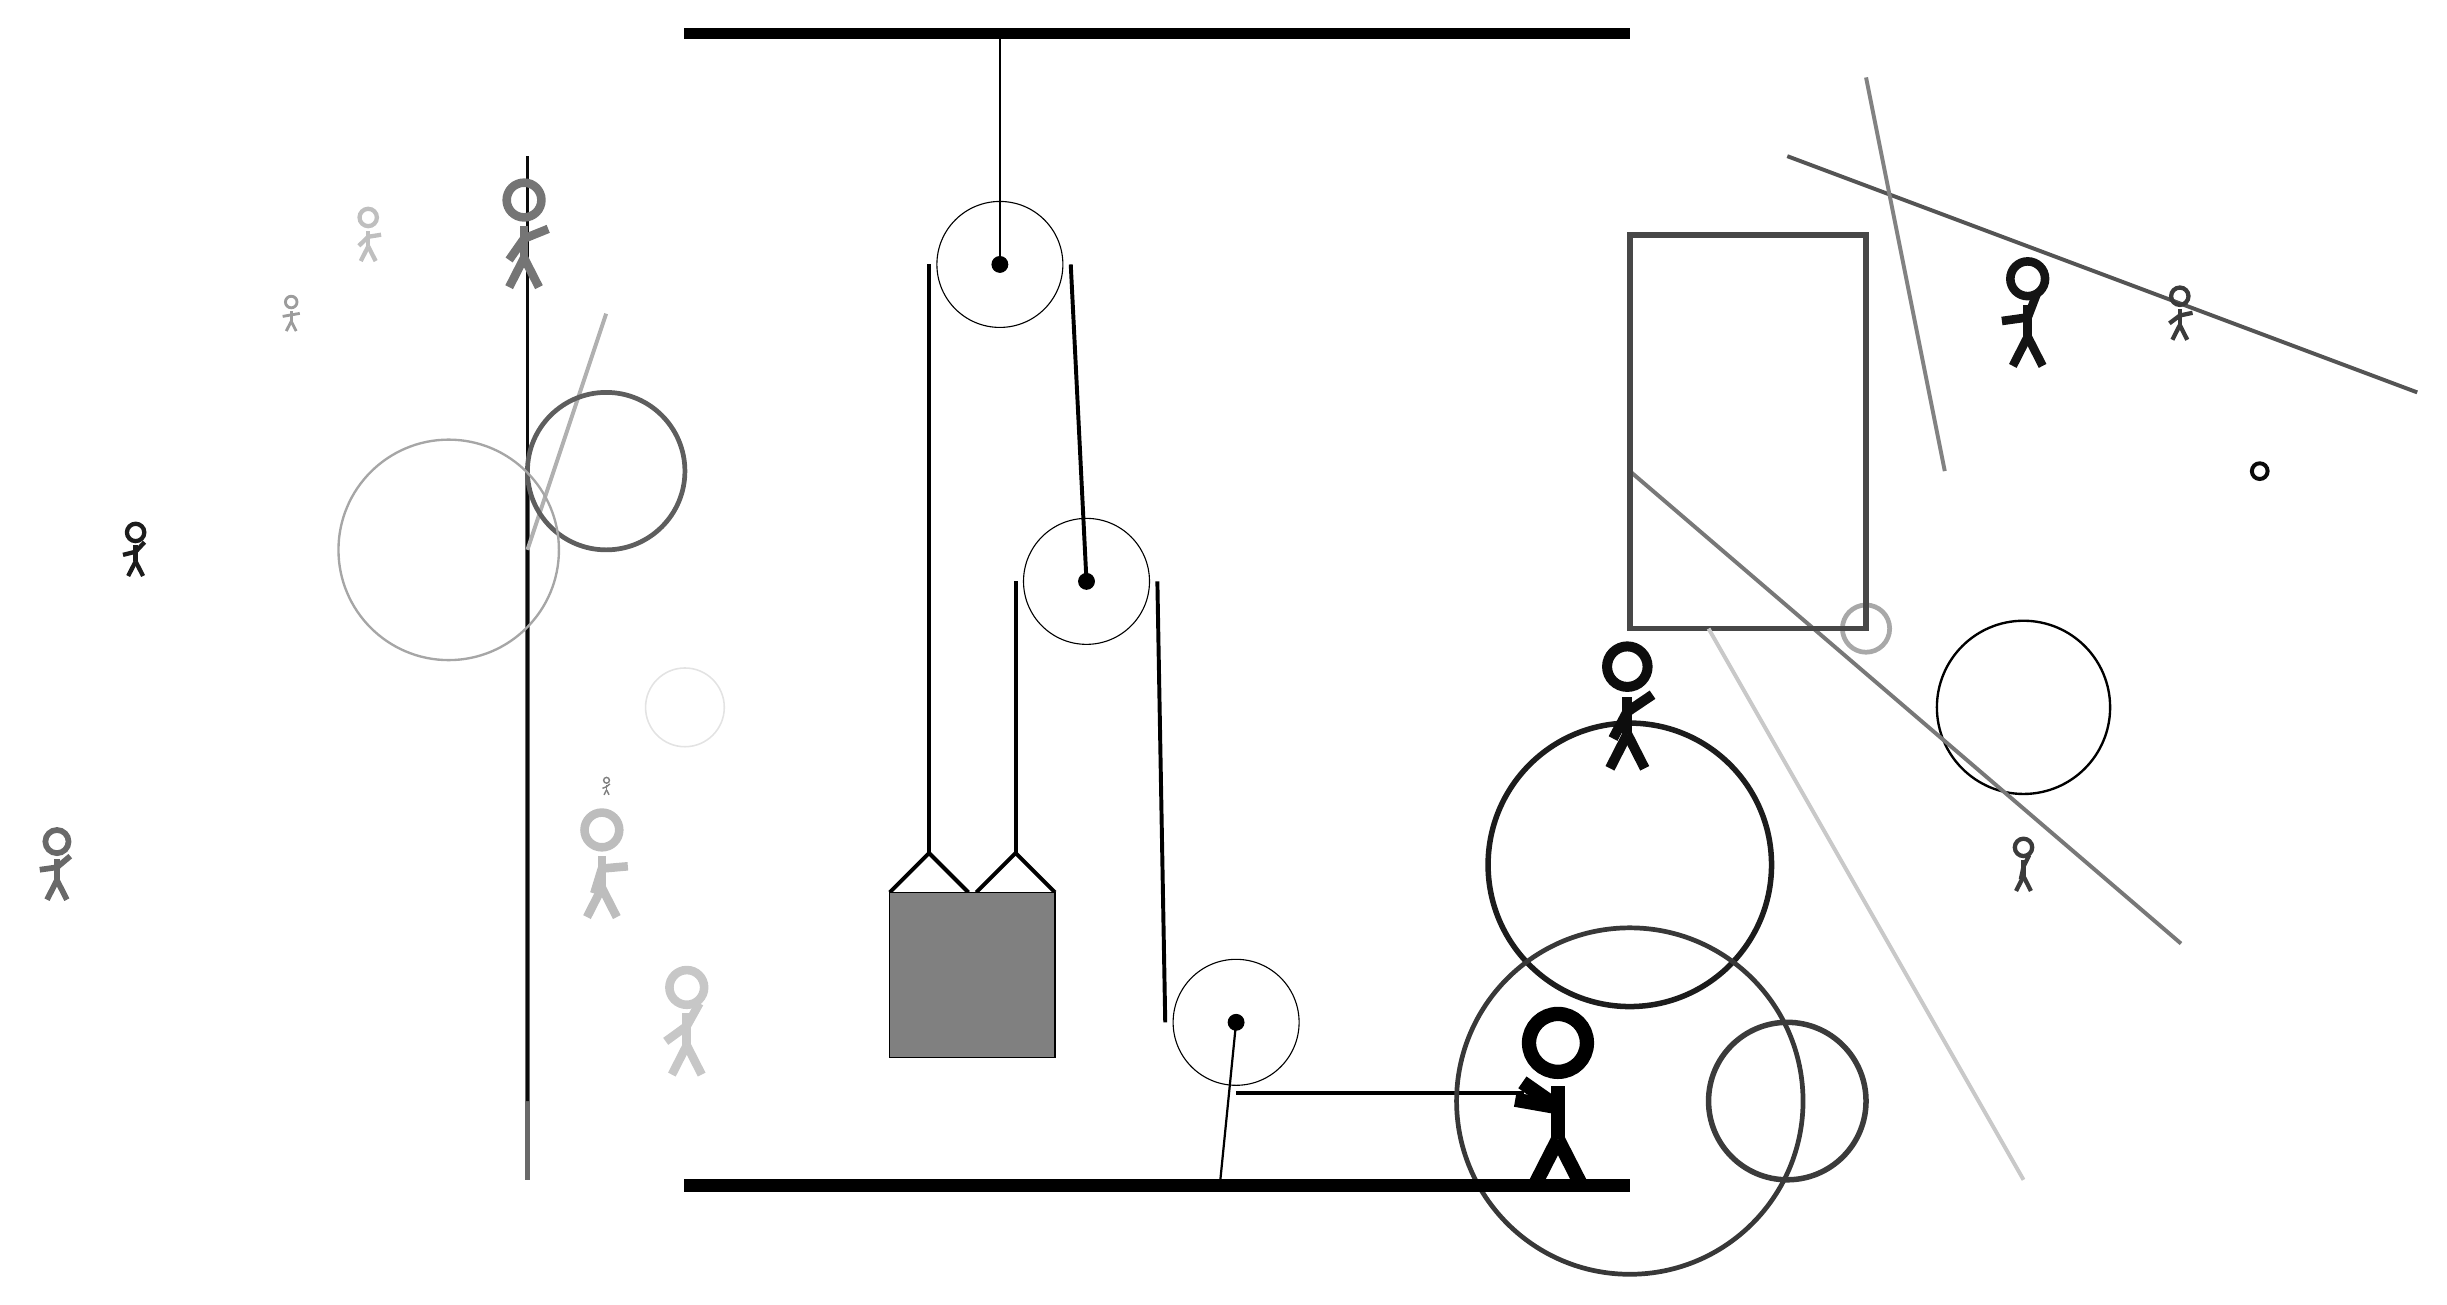
\begin{tikzpicture}
			%%%%% START %%%%%
			
			\draw[fill=black] (-2, 11.5) rectangle (10, 11.625);
			
			\draw (2, 8.625) circle (0.8);
			\draw[fill=black] (2, 8.625) circle (0.1);
			\draw[thick] (2, 8.625) -- (2, 11.5);
			
			\draw (3.1, 4.6) circle (0.8);
			\draw[fill=black] (3.1, 4.6) circle (0.1);
			
			\draw (5, -1) circle (0.8);
			\draw[fill=black] (5, -1) circle (0.1);
			\draw[thick] (5, -1) -- (4.8, -3);
			
			\draw[line width = 0.5mm]  (0.6, 0.65) -- (1.1, 1.15) -- (1.6, 0.65);
			\draw[line width = 0.5mm]  (1.7, 0.65) -- (2.2, 1.15) -- (2.7, 0.65);
			\draw[fill=black!50] (0.6, 0.65) rectangle (2.7, -1.45);
			
			\draw[line width = 0.5mm] (1.1, 8.625) -- (1.1, 1.15);
			\centerarc[line width = 0.5mm](2, 8.625)(0:180:0.9);
			\draw[line width = 0.5mm] (2.9, 8.625) -- (3.1, 4.6);
			\draw[line width = 0.5mm] (2.2, 4.6) -- (2.2, 1.15);
			\centerarc[line width = 0.5mm](3.1, 4.6)(0:180:0.9);
			\draw[line width = 0.5mm] (4.0, 4.6) -- (4.1, -1);
			\centerarc[line width = 0.5mm](5, -1)(180:270:0.9);
			\draw[line width = 0.5mm] (5, -1.9) -- (8.65, -1.9);
			
			\node at (9, -2) {\Strichmaxerl[10][-35][170]};
			
			\draw [line width=0.3mm, color=black!100](15, 3) circle (1.1);
			
			\draw[line width=0.7mm, color=black!59] (-4, -3) rectangle (-4, 6);
			\draw [line width=0.7mm, color=black!89](10, 1) circle (1.8);
			\draw[line width=0.3mm, color=black!96] (-4, -2) rectangle (-4, 10);
			\node[line width=0.2mm, color=black!25] at (-6, 9) {\Strichmaxerl[3][44][9]};
			\node[line width=0.3mm, color=black!54] at (-4, 9) {\Strichmaxerl[6][55][22]};
			\node[line width=0.2mm, color=black!22] at (-2, -1) {\Strichmaxerl[6][36][61]};
			
			\node[line width=0.7mm, color=black!89] at (-9, 5) {\Strichmaxerl[3][14][47]};
			\node[line width=0.5mm, color=black!26] at (-3, 1) {\Strichmaxerl[6][73][5]};
			\node[line width=0.7mm, color=black!59] at (-10, 1) {\Strichmaxerl[4][8][40]};
			
			\draw [line width=0.5mm, color=black!96](18, 6) circle (0.1);
			\draw [line width=0.2mm, color=black!11](-2, 3) circle (0.5);
			\draw[line width=0.5mm, color=black!31](-4, 5) -- (-3, 8);
			
			\node[line width=0.2mm, color=black!95] at (10, 3) {\Strichmaxerl[7][62][34]};
			\draw [line width=0.6mm, color=black!78](10, -2) circle (2.2);
			\draw [line width=0.6mm, color=black!34](13, 4) circle (0.3);
			\draw[line width=0.5mm, color=black!67](12, 10) -- (20, 7);
			
			\draw [line width=0.6mm, color=black!63](-3, 6) circle (1.0);
			\node[line width=0.4mm, color=black!77] at (15, 1) {\Strichmaxerl[3][78][64]};
			\node[line width=0.6mm, color=black!50] at (-3, 2) {\Strichmaxerl[1][22][40]};
			\draw[line width=0.5mm, color=black!53](10, 6) -- (17, 0);
			
			\node[line width=0.6mm, color=black!39] at (-7, 8) {\Strichmaxerl[2][10][10]};
			
			\node[line width=0.7mm, color=black!77] at (17, 8) {\Strichmaxerl[3][37][12]};
			\draw[line width=0.7mm, color=black!72] (10, 4) rectangle (13, 9);
			\draw [line width=0.3mm, color=black!35](-5, 5) circle (1.4);
			
			\node[line width=0.3mm, color=black!92] at (15, 8) {\Strichmaxerl[6][8][69]};
			\draw [line width=0.7mm, color=black!77](12, -2) circle (1.0);
			\draw[line width=0.5mm, color=black!49](13, 11) -- (14, 6);
			
			\draw[line width=0.5mm, color=black!21](11, 4) -- (15, -3);
			
			
			\draw[fill=black] (-2, -3) rectangle (10, -3.15);
			
			%%%%% END %%%%%
		\end{tikzpicture}
	\end{figure}	
\end{document}